\section{Comparing Models on Full Statistics Signal}
So far in the analysis I have only tested on a subset of the signal, which I have called the original signal set. In this section 
I will extend my search to include the full signal set displayed in figure \ref{fig:nrSignal}. The full signal set consists of 89 mass 
combinations compared to the original 30, and extends the mass ranges to $\tilde{\chi}_1 \in [0-400]GeV$ and $\tilde{\chi}_2 \in [200-800]GeV$.
In the figures to come, I have included a turquoise band around all combinations with a significance of over 1.64 (see section \ref{subsec:Sensitivity}).
When comparing the results, we are not only interested in how sensitive the models are for each combination individually, but also with how many combinations 
they were able to achieve a sensitivity of over 1.64. However, similarly to previous results, the significance does not include any uncertainty.
\\
\begin{figure}
    \makebox[\linewidth][c]{%
    \centering
    \begin{subfigure}{.85\textwidth}
        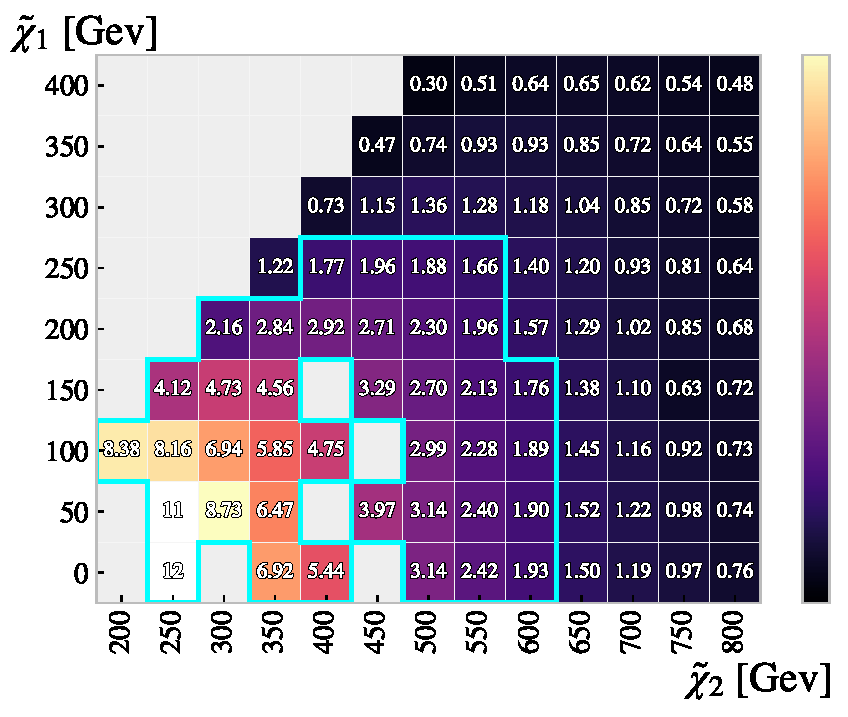
\includegraphics[width=\textwidth]{Figures/MLResults/NN/SUSY/Grid/FS/NN_FS_MLMGridSig.pdf}
    \end{subfigure}
    }
    \caption{A grid displaying the achieved significance on the full statistics signal set, using the signal region 
    created by the \emph{NN} network.}
    \label{fig:NN_FS_MLMGridSig}
\end{figure}

\begin{figure}
    \makebox[\linewidth][c]{%
    \centering
    \begin{subfigure}{.85\textwidth}
        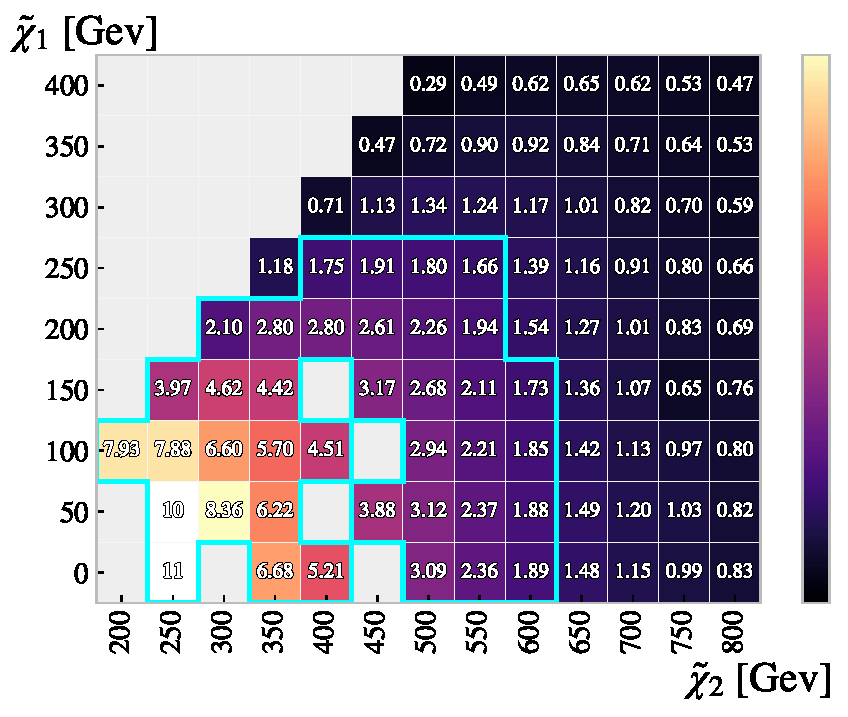
\includegraphics[width=\textwidth]{Figures/MLResults/NN/SUSY/Grid/FS/MaxOutPCA_FS_MLMGridSig.pdf}
    \end{subfigure}
    }
    \caption{A grid displaying the achieved significance on the full statistics signal set, using the signal region 
    created by the \emph{MaxOut} network.}
    \label{fig:MaxOutPCA_FS_MLMGridSig}
\end{figure}

\begin{figure}
    \makebox[\linewidth][c]{%
    \centering
    \begin{subfigure}{.85\textwidth}
        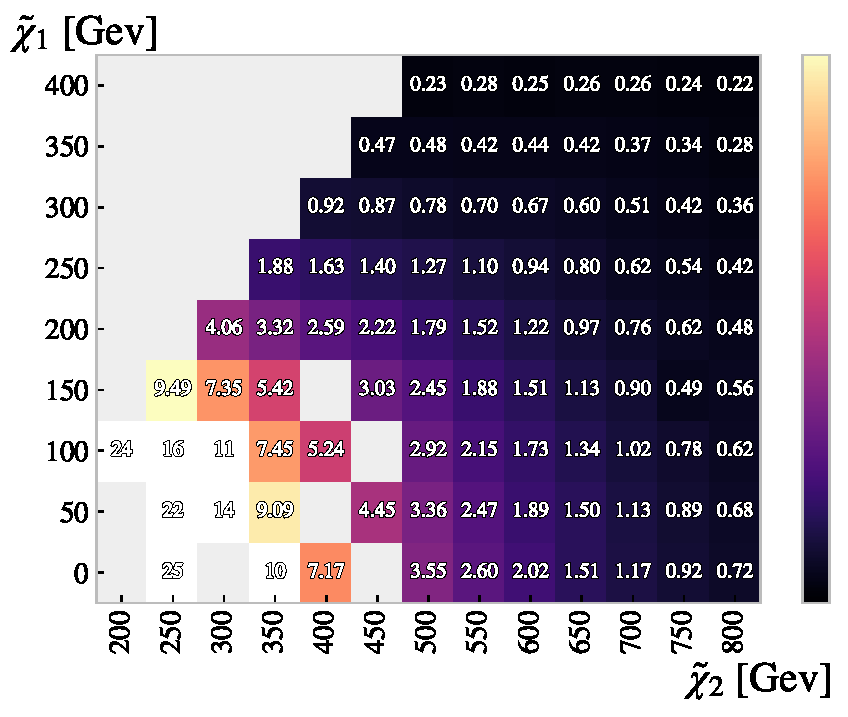
\includegraphics[width=\textwidth]{Figures/MLResults/NN/SUSY/Grid/FS/PNNPCA_FS_MLMGridSig.pdf}
    \end{subfigure}
    }
    \caption{A grid displaying the achieved significance on the full statistics signal set, using the signal region 
    created by the \emph{PNN} network.}
    \label{fig:PNNPCA_FS_MLMGridSig}
\end{figure}